\chapter{Reinforcement Learning}

Beim verst�rkenden Lernen geht es darum, ein Modell anhand von Konsequenzen zu trainieren, d. H. Belohnungen oder Bestrafungen, basierend auf Aktionen, die das Modell ausf�hrt. Dieses positive oder negative Feedback wird dann vom Modell verwendet, um �ber zuk�nftige Aktionen zu entscheiden.

\section{Lernen durch positives und negatives Feedback}

Das allgemeine Ziel eines Modells, das diese Art des Lernens durchl�uft, ist, dass es entweder ``�berlebt'' oder von erfolgreichen Reaktionen gewinnen. Das genauere Ziel des Modales ist es, eine �berlebens- oder Gewinnstrategie (engl. Policy) zu entwickeln, um die erhaltenen Belohnungen zu maximieren.

Der Lerner wei� zun�chst nichts dar�ber, was vor ihm liegt und was ihn vor der Exploration erwartet. Der Lernende muss sich also entscheiden, ob er einen neuen Zustand erkunden oder in einen bereits bekannten Zustand �bergehen soll.

\paragraph{Lernstrategiebeispiel:}

\begin{enumerate}
    \item Lerner befindet sich in einem Zustand \(s_i\) in einem \textbf{diskreten} Zustandsraum \(\Sigma\).
    \item Der Lerner versucht dann, ein oder mehrere Ziele zu erreichen.
    \item Im Zustand \(s_i\) kann der Lernende aus einer Reihe von auszuf�hrenden Aktionen \(A=\{a_{i,1}, \ldots, a_{a,n}\}\) w�hlen.
    \item Von der Ausf�hrung der Aktion \(a_{i,k}\) bewegt sich der Lerner zum n�chsten Zustand.
    \item Im n�chsten Zustand erh�lt der Lerner eine Belohnung oder Bestrafung, je nachdem, wie gut die Handlung dazu beigetragen hat, das Ziel zu erreichen.
\end{enumerate}

Dies wirft nat�rlich die Frage auf: Wie soll das Modell im Zustand \(s_i\) die beste Aktion, \(a\) ausw�hlen? In diesem Fall wird nach der Funktion \(f^\pi\) gesucht, die basierend auf dem aktuellen Zustand \(s_i\) die beste Aktion \(a_{i,k}\) empfiehlt: \[f^\pi:\Sigma \rightarrow A \textnormal{ mit } f^\pi(s_i)=a_{i,k} \]

In dieser Notation stellt \(\pi\) eine Abfolge von Aktionen (Strategie oder Policy) dar, die mit \(f^\pi\) bestimmt wird. \(f^\pi\) kann als eine Lookup-Tabelle implementiert werden. 

Ein alternativer Ansatz w�re, die Erfolgsaussichten der Durchf�hrung einer Aktion \(a_{i,k}\) in Zustand \(s_i\) zu bestimmen. Daf�r gibt es zwei Varianten:

\begin{itemize}
    \item \textbf{Value-Funktion:} \(V^\pi(s) \rightarrow w \in IR\). Wenn die Policy \(\pi\) im Zustand \(s\) befolgt wird, wird die Belohnung \(w\) erhalten.
    \item \textbf{Q-Funktion:} \(Q^\pi(s,a) \rightarrow w \in IR\). Wenn die Policy \(\pi\) im Zustand \(s\) befolgt wird, wird die Belohnung \(w\) erhalten. Der Vorteil des Q-Wertes ist, dass er als Entscheidungshilfe dient, um auszuw�hlen, welche verf�gbare Aktion, \(a_{i,k}\) im Zustand \(s_i\).
\end{itemize}

\section{Der Q-Learning Ansatz}

Q-Learning ist ein Ansatz, um die optimale Policy \(\pi\) zu finden. Dies wird iterativ durchgef�hrt, um die Funktion \(Q^\pi(s,a) \rightarrow w \in IR\) zu approximieren. In jedem Iterationsschritt wird ein Zustand-Aktions-Paar in einer Tabelle gem�� der folgenden Q-Update-Regel aktualisiert:

\[Q(s_{i_{new}}, a_{j_{new}}) = Q(s_{i_{old}}, a_{j_{old}}) + \alpha * (r(s_i, a_j) + \gamma * max_k\{Q(s_{i+k}, a_k)\} - Q(s_{i_{old}}, a_{j_{old}}))\]

wobei \(\alpha\) die Lernrate, \(r\) die Belohnung im Zustand \(s_i\), wenn Aktion \(a_i\) ausgef�hrt wird, \(\gamma\) der ``Discount''-parameter zur Gewichtung des Look Ahead und \(Q\) die Look-Ahead-Funktion f�r zuk�nftige Belohnungen sind.

Die Aktionszustandspaare werden in einer Tabelle gespeichert, die als \textbf{Q-Tabelle} bekannt ist, die meist als geschachteltes Array implementiert ist. Die Q-Tabelle wird w�hrend des Lernprozesses iterativ aktualisiert, um eine Tabelle mit aussagekr�ftigen Werten f�r jede Aktion basierend auf dem aktuellen Zustand zu erhalten.

Q-Learning erfordert viel Aufwand, aber es hat sich gezeigt, dass, wenn die Anzahl der Iterationen gegen unendlich wird, die durch Q-Learning gefundene Richtlinie zur optimalen Strategie f�r die gegebenen Zustandsaktionspaare konvergiert.

In der Praxis ist es jedoch nicht m�glich, ewig zu trainieren, daher sind Abbruchkriterien erforderlich: Abbruch nach definierter Anzahl von ITerationen, Abbruch wenn nur noch kleine �nderungen beim Update erzielt werden oder Abbruch, die bis dato gelernter Strategie das Problem ann�hernd l�st.

Unter Verwendung der erlernten Q-Tabelle wird die beste Aktion f�r jeden Zustand basierend auf der Aktion mit dem h�chsten Q-Wert ausgew�hlt. So wird Q-learning durchgef�hrt.

\subsection{Steuerung des Lernverfahrens}

Abgesehen von der Anzahl der Epochen k�nnen die in der Q-Update-Regel enthaltenen Parameter \(\alpha\) und \(\alpha\) den Lernprozess beeinflussen.

\paragraph{Lernrate, \(\alpha\)}

Der Wert von \(\alpha\) muss zwischen 1 und 0 liegen. Ein zu gro�er Wert (\(\alpha \sim 1\)) k�nnte dazu f�hren, dass die Q-Funktion zu grob angen�hert wird. W�hlen Sie einen zu kleinen Alpha-Wert, (\(\alpha \sim 0\)), dann ben�tigt der Trainingsprozess mehr Zeit.

\paragraph{Discountfaktor, \(\gamma\)}

Der Wert von \(\gamma\) steuert, wie wichtig die Vorausschau auf das Ergebnis der Regel ist. Ohne Look-Ahead w�rden nur lokale Bewertungen ber�cksichtigt und keine globale Strategie gelernt. Daher wird normalerweise ein Wert von 0,8 bis 0,95 gew�hlt. Wenn der Wert jedoch zu gro� ist, kann dies den Belohnungswert �berschatten, was nicht erw�nscht ist.

\subsection{Rolle des Zufalls beim Q-Learning}

Bei der erstmaligen Initialisierung der Werte der Q-Tabelle kann es vorteilhaft sein, diese auf Zufallswerte zu initialisieren. Auf diese Weise kann es sein, dass einige der Werte bereits nahe am idealen Wert der Ann�herung liegen. Alternativ werden die Werte alle mit demselben festen Wert initialisiert.

In der Q-learn-Regel soll der Term \(max_k\{Q(s_{i+k}, a_k)\}\) die am besten bewertete Aktion im Vorausschauen ausw�hlen. Dies ist als ``greedy''-Ansatz bekannt und kann dazu f�hren, dass bessere globale Strategien �bersehen werden. Um dies zu �berwinden, wird \(\epsilon\textnormal{-soft}\) verwendet. Das bedeutet, dass in 1 bis \(\epsilon\) \% der F�lle, die gew�hlte Look-Ahead-Aktion zuf�llig ausgew�hlt wird.

\subsection{Bewertung von Q-Learning}

\section{Veretiefungsprojekt: Q-Learning mit OpenAI Gym}

Zur Vertiefung des Kapitels wurde das Q-Learning mit Python und OpenAI Gym implementiert. Die Umsetzung erfolgte auf der Grundlage eines Online-Artikels von learndatasci.com\cite{q-learning-article}. In diesem Beispiel wurde die OpenAI Gym-Umgebung ``Taxi-v3'' verwendet, die die Zust�nde, Aktionen und Belohnungen f�r den Q-Learning-Algorithmus und das Rendering der Zustandsdarstellung bereitstellt. Der vollst�ndige Code des Programms ist unter vertiefungen-projekte/python/reinforcement-learning/ zu finden.

\begin{figure}[H]
    \centering
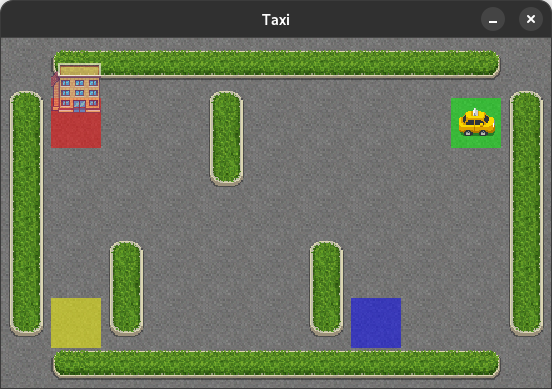
\includegraphics[width=0.7\textwidth]{figures/kap14/vertiefung-qlearning.png}
    \caption{Screenshot der trainierten KI}
    \label{fig:q-learning-screenshot}
\end{figure}

\subsection{Ausf�hren des Programms}
Um das Programm auszuf�hren:
\begin{enumerate}
    \item Zum Ordner navigieren: vertiefungen-projekte/python/reinforcement-learning/
    \item F�hre Folgendes in einem Terminal aus
\begin{lstlisting}[language=bash]
# install dependencies
pip install -r requirements.txt

# run program
python3 taxi-qlearning.py
\end{lstlisting}
\end{enumerate}

\subsection{�berblick �ber den Ablauf}
Das Programm beginnt mit der Erstellung der OpenAI Gym-Umgebung und der Initialisierung einer leeren Q-Tabelle. Das Programm beginnt mit der Erstellung der OpenAI Gym-Umgebung und der Initialisierung einer leeren Q-Tabelle.

\begin{lstlisting}[language=python]
env = gym.make("Taxi-v3").env
q_table = np.zeros([env.observation_space.n,env.action_space.n])
\end{lstlisting}

Die Parameter f�r die Q-Regel werden dann wie folgt festgelegt.

\begin{lstlisting}[language=python]
# Q-Regel parameters
alpha = 0.1
gamma = 0.6
epsilon = 0.1
\end{lstlisting}

Das Training beginnt dann f�r jede Epoche in der While-Schleife. Zu Beginn einer Epoche wird ein zuf�lliger Wert gegen Epsilon gepr�ft, um zu entscheiden, ob der Aktionsraum erkundet oder bereits erlernte Werte ausgenutzt werden sollen.

\begin{lstlisting}[language=python]
while not epoch_done:
if random.uniform(0, 1) < epsilon:
    action = env.action_space.sample() # Explore action space
else:
    action = np.argmax(q_table[state]) # Exploit learned values
\end{lstlisting}

Dann wird eine Aktion durchgef�hrt (entweder aus der Q-Tabelle oder aus der Umgebung) und die Q-Tabelle wird unter Verwendung der Q-Regelgleichung aktualisiert.

\begin{lstlisting}[language=python]
next_state, reward, epoch_done, info = env.step(action) 

old_value = q_table[state, action]
next_max = np.max(q_table[next_state])

new_value = (1 - alpha) * old_value + alpha * (reward + gamma * next_max)
q_table[state, action] = new_value
\end{lstlisting}

Dies wird f�r jede Epoche in jeder Episode durchgef�hrt, bis das Training abgeschlossen ist. Schlie�lich wird das trainierte Modell getestet (und gerendert), um zu beobachten, wie gut es trainiert wurde. 